\documentclass[titlepage, a4paper, 12pt, reqno, openany]{report}
%\documentclass[12pt]{report}
%\documentclass[titlepage, a4paper, 12pt, reqno, openany]{article}
%\documentclass[12pt]{article}
%%%%%%%%%%%%%%%%%%%%%%%%%%%%%%%%%%%%%%%%%%%%%%%%%%%%%%%%%%%%%%%%%%%%%%%%%%%%%
\usepackage{titlepic}
%%%%%%encoding%%%%%%
\usepackage[T1]{fontenc}
\usepackage[utf8]{inputenc}
\usepackage[portuguese]{babel}
\usepackage{hyphenat}
%\usepackage{hyphsubst}
%%%%%%Hyphenation rules%%%%%%
\usepackage{graphicx} %permite inserir figuras
\usepackage{caption} %titulo graphicos
\usepackage[font=small,labelfont=bf]{caption} %reference figures
%\usepackage{subcaption}
\usepackage{color,colortbl}
\usepackage[usenames,dvipsnames,svgnames,table]{xcolor} %permite letras coloridas
\usepackage[top=2cm,left=1.5cm,right=1.2cm,bottom=2cm]{geometry}
%\usepackage[margin=2cm]{geometry} %margens
%\usepackage[left=2cm,top=1cm,bottom=2cm,right=3cm,nohead,nofoot]{geometry}
\usepackage{paralist}
\usepackage{float}
\usepackage{verbatim}
\usepackage{lipsum}
\usepackage{multicol}
\usepackage{multirow}
\usepackage{makecell}
\usepackage{babelbib}
%\usepackage{biblatex}
\usepackage{amsfonts}
\usepackage{amsmath}
\usepackage{amssymb}
%%%%%%%%%%%%%%%%%%%%%%%%%%%%%%%%%%%%%%%%%%%%%%%%%%%%%%%%%%%%%%%%%%%%%%%%%%%%%%%
\usepackage[export]{adjustbox}
\usepackage{lipsum}
%\usepackage{adjustbox}
\usepackage{setspace} %distancia entree linhas
\usepackage{eurosym}
%\usepackage[table,xcdraw]{xcolor}
%\usepackage{times}
%\usepackage{makeidx} %para criar índice remissivo
%\usepackage{array}
%\usepackage{supertabular}
%\usepackage{bm}
%\usepackage{booktabs}
%\usepackage{boxedminipage}
%\usepackage{caption}
%\usepackage{changepage}
%\usepackage{cite}
%\usepackage{easylist}
%\usepackage{esint}
%\usepackage{eucal}
%\usepackage{fancyhdr}
%\usepackage{hyperref} %index dentro de red boxes
%\usepackage{indentfirst}
%\usepackage{latexsym}
%\usepackage{listings}
%\usepackage{mathptmx}
%\usepackage{mathrsfs} %permite o uso de letras trabalhadas
%\usepackage{microtype}
%\usepackage[normalem]{ulem} %permite sublinhar palavras
%\usepackage{pifont}
%\usepackage{rotating}
%\usepackage{setspace}
%\usepackage{syntonly} %speedup work desabling pdf converse \syntaxonly
%\usepackage{subfiles}
%\usepackage{textcomp}
%\usepackage{theorem}
%\usepackage{ulem}
%\usepackage{url}
%\usepackage{wrapfig}
%%%%%recent%%%%%
%\usepackage{cancel}
%\usepackage[fleqn]{mathtools}
%\usepackage{pdfpages}
%\usepackage{pdflscape}
%\usepackage{todonotes}
%\usepackage{siunitx}
%%%%%%%%%%%%%%%%%%%%%%%%%%%%%%%%%%%%%%%%%%%%%%%%%%%%%%%%%%%%%%%%%%%%%%%%%%%%%%%%%%%
%\renewcommand\thesection{\arabic{section}}
%\renewcommand\thesubsection{\thesection.\arabic{subsection}}
%%%%%%%%%%%%%%%%%%%%%%%%%%%%%%%%%%%%%%%%%%%%%%%%%%%%%%%%%%%%%%%%%%%%%%%%%%%%%%%%%%%%
\usepackage{enumitem}
\begin{comment}
\setlistdepth{12}
\newlist{enumitem}{enumerate}{12}
\setlist[enumitem,1]{label=\roman*)}
\setlist[enumitem,2]{label=\alph*)}
\setlist[enumitem,3]{label=\arabic*)}
\setlist[enumitem,4]{label=(\roman*)}
\setlist[enumitem,5]{label=(\alph*)}
\setlist[enumitem,6]{label=(\arabic*)}
\setlist[enumitem,7]{label=\roman*)}
\setlist[enumitem,8]{label=\alph*)}
\setlist[enumitem,9]{label=\arabic*)}
\setlist[enumitem,10]{label=(\roman*)}
\setlist[enumitem,11]{label=(\alph*)}
\setlist[enumitem,12]{label=(\arabic*)}
\end{comment}

%%%%%%%%%%%%%%%%%%%%%%%%%%%%%%%%%%%%%%%%%%%%%%%%%%%%%%%%%%%%%%%%%%%%%%%%%%%%%%%%%%%%
\begin{comment}
\usepackage{enumerate}
\renewcommand{\labelitemi}{$\bullet$}
\renewcommand{\labelitemii}{$\cdot$}
\renewcommand{\labelitemiii}{$\diamond$}
\renewcommand{\labelitemiv}{$\ast$}
\end{comment}

%%%%%%%%%%%%%%%%%%%%%%%%%%%%%%%%%%%%%%%%%%%%%%%%%%%%%%%%%%%%%%%%%%%%%%%%%%%%%%%%%%%%
\begin{comment}
\usepackage{tikz}
\usepackage{circuitikz}
\usetikzlibrary{matrix,shapes.geometric,arrows,trees,positioning,calc}
%%%%%%%%%%%%%%%%%%%%%%%pre defined figures%%%%%%%%%%%%%%%%%%%%%
\tikzstyle{RECTANGLE_2} = [rectangle, draw, text width=5em, text centered, rounded corners, minimum height=4em]
\tikzstyle{RECTANGLE_3} = [rectangle, rounded corners, minimum width=3cm, minimum height=1cm,text centered, draw=black, fill=red!80]
\tikzstyle{RECTANGLE_4} = [rectangle, draw, fill=blue!20, text width=3cm, text centered, minimum height=4em]
\tikzstyle{RECTANGLE_5} = [rectangle, minimum width=3cm, minimum height=1cm, text centered, text width=3cm]
\tikzstyle{RECTANGLE_6} = [rectangle, draw, fill=blue!20, text width=5em, text centered, rounded corners, minimum height=4em]
\tikzstyle{RECTANGLE_7} = [rectangle, draw, fill=blue!20, text width=5em, text centered, rounded corners, minimum height=4em]
\tikzstyle{RECTANGLE_8} = [rectangle, draw, align=left, fill=blue!20]
\tikzstyle{RECTANGLE_1} = [rectangle, rounded corners, minimum width=1cm, minimum height=1cm,text centered, draw=black, fill=green!%30]
\tikzstyle{DIAMOND_1} = [diamond, draw, fill=blue!20, text width=4.5em, text badly centered, node distance=4cm, inner sep=0pt]
\tikzstyle{DIAMOND_2} = [diamond, minimum width=3cm, minimum height=1cm, text centered, draw=black, fill=green!30]
\tikzstyle{DIAMOND_3} = [diamond, draw, text width=4.5em, text badly centered, node distance=3cm, inner sep=0pt]
\tikzstyle{DIAMOND_4} = [diamond, draw, fill=blue!20, text width=4.5em, text badly centered, node distance=3cm, inner sep=0pt]
\tikzstyle{DIAMOND_5} = [diamond, draw, fill=blue!20, text width=4.5em, text badly centered, node distance=3cm, inner sep=0pt]
\tikzstyle{DIAMOND_6} = [diamond, draw, fill=blue!20, text width=4.5em, text badly centered, node distance=4cm, inner sep=0pt]
\tikzstyle{DIAMOND_7} = [diamond, draw, align=left, fill=blue!20]
\tikzstyle{ELLIPSE_1} = [draw, ellipse,fill=red!20, node distance=3cm, minimum height=2em]
\tikzstyle{ELLIPSE_2} = [draw, ellipse,fill=red!20, node distance=3cm, minimum height=2em]
\tikzstyle{ELLIPSE} = [draw, ellipse,fill=red!20, node distance=3cm, minimum height=2em]
\tikzstyle{TRAPEZIUM_1} = [trapezium,trapezium left angle=70,trapezium right angle=-70,minimum height=0.6cm, draw, fill=blue!20, text width=4.5em, text badly centered, node distance=3cm, inner sep=0pt]
\tikzstyle{TRAPEZIUM_2} = [trapezium, trapezium left angle=70, trapezium right angle=110, minimum width=3cm, minimum height=1cm, text centered, draw=black, fill=blue!30]
\tikzstyle{TRAPEZIUM_3} = [trapezium,trapezium left angle=70,trapezium right angle=-70,minimum height=0.6cm, draw, fill=blue!20, text width=4.5em, text badly centered, node distance=3cm, inner sep=0pt]
\tikzstyle{ARROW} = [thick,->,>=stealth]
\tikzstyle{LINE} = [draw, -latex']
\tikzstyle{MYLINE} = [draw, ->,  thick, shorten <=4pt, shorten >=4pt]
\tikzstyle{TEXT_1}=[draw,text centered,minimum size=6em,text width=5.25cm,text height=0.34cm]
\tikzstyle{TEXT_2}=[draw,text centered,minimum size=2em,text width=2.75cm,text height=0.34cm]
\tikzstyle{TEXT_3}=[draw,minimum size=2.5em,text centered,text width=3.5cm]
\tikzstyle{TEXT_4}=[draw,minimum size=3em,text centered,text width=6.cm]
\tikzstyle{CIRCLE_1}=[draw,shape=circle,inner sep=2pt,text centered, node distance=3.5cm]
\tikzstyle{CIRCLE_2}=[draw,shape=circle,inner sep=4pt,text centered, node distance=3.cm]
\end{comment}

%%%%%%%%%%%%%%%%%%%%%%%%%%%%%%%%%Not Adviced%%%%%%%%%%%%%%%%%%%%%%%%%%%%%%%%%%%%%%%%
%\usepackage{showidx} %for troubleshooting index
%\usepackage{showkeys} %for troubleshooting \label \ref
%\usepackage{pxfonts}

%%%%%%%%%%%%%%%%%%%%%%%%%%%%%%%%%claching Package%%%%%%%%%%%%%%%%%%%%%%%%%%%%%%%%%%%
%\usepackage{pgfplots}
%\usepackage{natbib}
%\usepackage[usenames]{color} %permite letras coloridas
%\usepackage{xypic}

%%%%%%%%%%%%%%%%%%%%%%%%%%%%%%%%%Not Installed Yet%%%%%%%%%%%%%%%%%%%%%%%%%%%%%%%%%%

%%%%%%%%%%%%%%%%%%%%%%%%%%%%%%%Com Dependencias%%%%%%%%%%%%%%%%%%%%%%%%%%%%%%%%%%%%%
%\usepackage{glossaries}
%\usepackage[version=3]{mhchem}

%%%%%%%%%%%%%%%%%%%%%%%%%%%%%%%%%%%%%%%%%%%%%%%%%%%%%%%%%%%%%%%%%%%%%%%%%%%%%%%%%%%%
% alguns pacotes nao sao reconhecidos, ter atencao quais usar em differents computadores, tambem alguns pacotes entram em conflito.
\newtheorem{theorem}{Theorem}
\newtheorem{lemma}{Lemma}
\newtheorem{definition}{Defini\c{c}\~{a}o}
\newtheorem{notation}{Notation}

%%%%%%%%%%%%%%%%%%%%%%%%%%%%%%%%Not Working%%%%%%%%%%%%%%%%%%%%%%%%%%%%%%%%%%%%%%%%%
%\usepackage{itemize}
%\usepackage{named}
%\usepackage{amscls}
%\usepackage{fullpage}

%%%%%%%%%%%%%%%%%%%%%%%%%%%%%%%%%%%%%%%%%%%%%%%%%%%%%%%%%%%%%%%%%%%%%%%%%%%%%%%%%%%%
%\usepackage{apacite} %Bibliography style
%%%%%%%%%%%%%%%%%%%%%%%%%%%%%%%%%%%%%%%%%%%%%%%%%%%%%%%%%%%%%%%%%%%%%%%%%%%%%%%%%%%%
\makeindex
%%%%%%%%%%%%%%%%%%%%%%%%%%%%%%%%%%%%%%%%%%%%%%%%%%%%%%%%%%%%%%%%%%%%%%%%%%%%%%%%%%%%



\begin{document}
%\bibliographystyle{apacite}
\bibliographystyle{babplain}
%\bibliographystyle{bstfilename}
%%%%%%%%%%FIX SECTION NUMBERING IN CASE REPORT%%%%%%%%%%%%
\renewcommand\thesection{\arabic{section}}
\renewcommand\thesubsection{\thesection.\arabic{subsection}}
\renewcommand\thesubsubsection{\thesection.\thesubsection.\arabic{subsubsection}}
%%%%%%%%%%%%%%%%%%%%%%%%%%%%%%%%%%%%%%%%%%%%%%%%%%%%%%%%%%
{\Huge \bf Trabalho 3 Prep} \\
\\
{\Large
\hspace*{1.5cm}{\bf Nome: Sérgio Santos} \\
\\
\hspace*{1.5cm}{\bf nº: 1020881}\\
}
\section{Esquema}
\begin{figure}[H]
	\centering
	\includegraphics[scale=0.7]{./image/esquema.jpg}\\
	\caption{Esquema}
\end{figure}
Um condensador quando esta a ser alimentado por uma fonte de corrente com um valor constante este carrega de forma linear no tempo, sendo que a corrente fornecida determina sua taxa de crescimentos, $\left[ \frac{Volt}{Sec} \right]$.\\ \\
O circuito alimentado com uma fonte de 19 Volt tem tensão de saída mínimo e máximo: \\
\begin{minipage}[l]{0pt}
	$$\left\lbrace\begin{array}{c}
 	-8,4 \quad V \\
 	9 \quad V \\
 \end{array}\right.$$
\end{minipage}
\hspace{3cm} 12,9 Kohm \qquad $\Longrightarrow$ \hspace{1cm}
\begin{minipage}[l]{0pt}
	$$\left\lbrace\begin{array}{c}
		6,5116 \times 10^{-4} \quad A \\
		6,9767 \times 10^{-4} \quad A \\
	\end{array}\right.$$
\end{minipage}\\
\\
\\
Vamos ver que o integrador vai usar um condensador de 1nF, que vai necessitar de uma corrente de carga de $6,96 \times 10^{-4} \quad A$, na qual traduz na resistência a ser usada, já que a malha de realimentação é uma fonte de corrente determinada pela resistência colocada na entrada inversor, é o principio de funcionamento do {\bf AMPOP} com realimentação negativa, mantém as entradas sempre ao mesmo potencial.
\begin{figure}[H]
	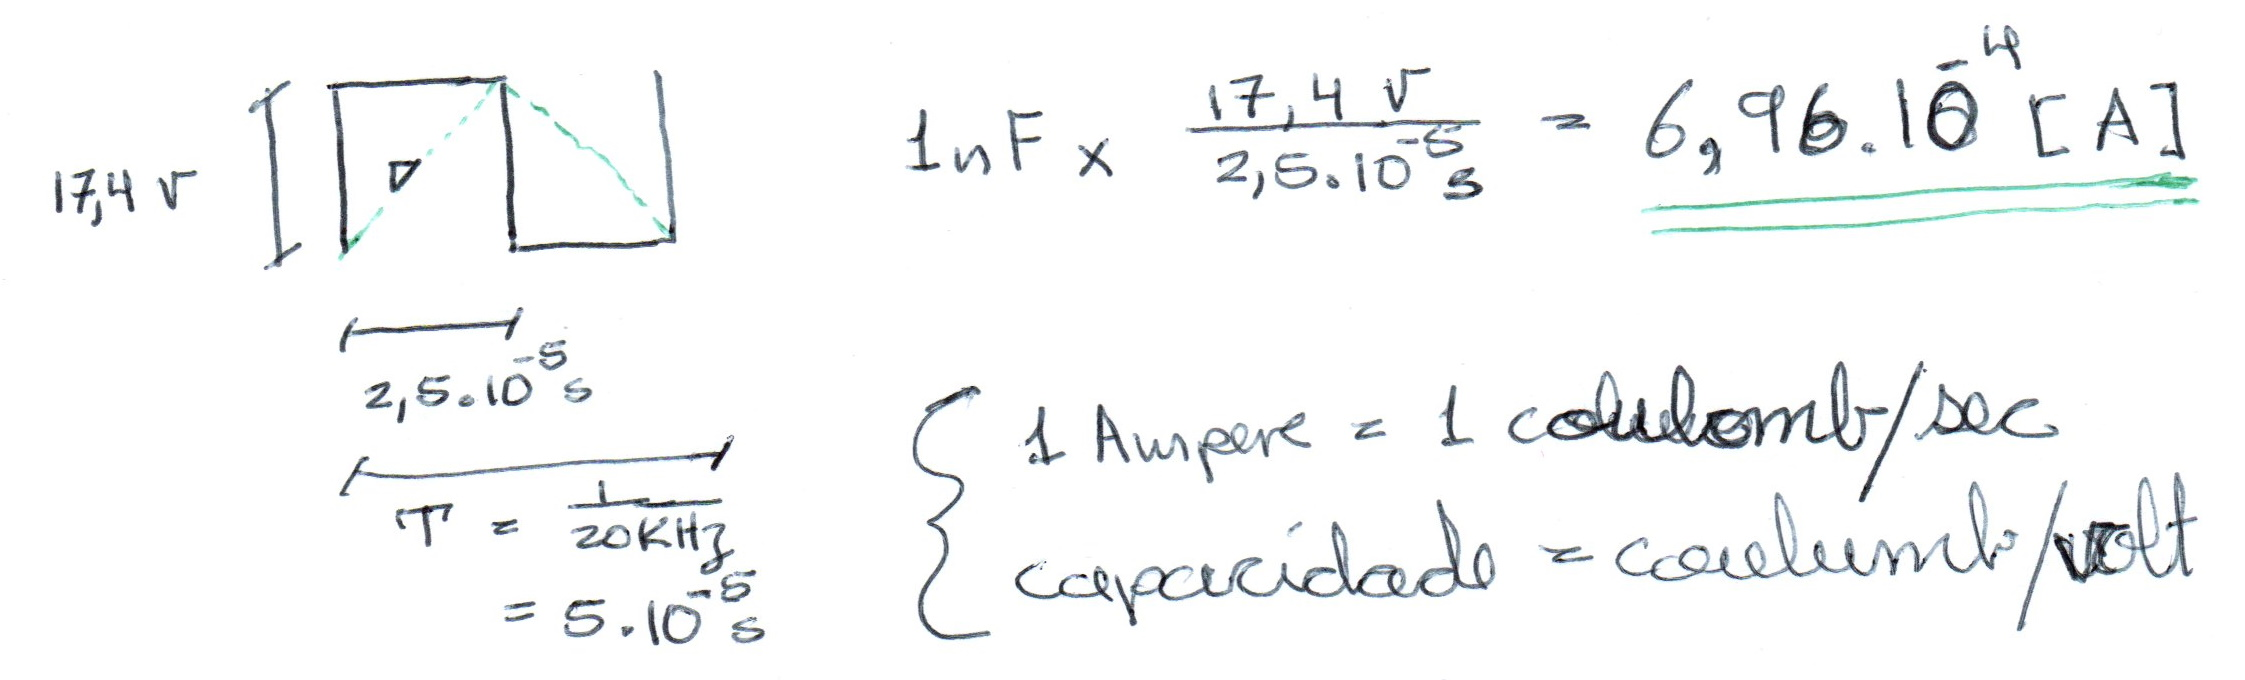
\includegraphics[scale=0.9]{./image/trb3calc_1.jpg}\\
	\caption{Determinar Corrente}
\end{figure}
%%%%%%%%%%%%%%%%%%%%%%%%%%%%%%%%%%%%%%%%%%%%%%%%%%%%%%%%%%%%%%%%%%%%%%%%%%%
\section{Material}
\begin{minipage}[t]{.4\linewidth}
	\begin{itemize}
		\setlength\itemsep{-0.5em}
		\item Resistencias \\
		1/4 Watt, varias.
		\item Potenciómetro multi-volta \\
		100Kohm e 1Kohm
		\item 7812 \\
		Regulador Tensão 12Volt
		\item Condensador \\
		1nF, 10nF  \\
		3x Eletrolítico 10uF
		
	\end{itemize}
\end{minipage}
\begin{minipage}[t]{.31\linewidth}
	%	\quad List 2:
	\begin{itemize}
		\setlength\itemsep{-0.5em}
		\item TL084 \\
		Quad Opamp Chip \\
		14 Pinos
		\item ICL7667 \\
		Dual Power MosFET Driver
		\item Ficha Alimentação
		\item Fusível 800mA
		\item Diodo 1N4148
		\item Led Verde \\
	\end{itemize}
\end{minipage}\\
\\
Circuito Funciona de 10 Volt até 32 Volt testado em bancada, sendo necessário ajuste fino para calibração pelo Potenciómetro de  1Kohm.
Pode se sempre consultar os {\it datasheets} dos componentes, na qual são todos visíveis na imagem.
\section{PCB (Printed Circuit Board)}
%\begin{comment}	
\begin{figure}[ht]
\begin{center}
	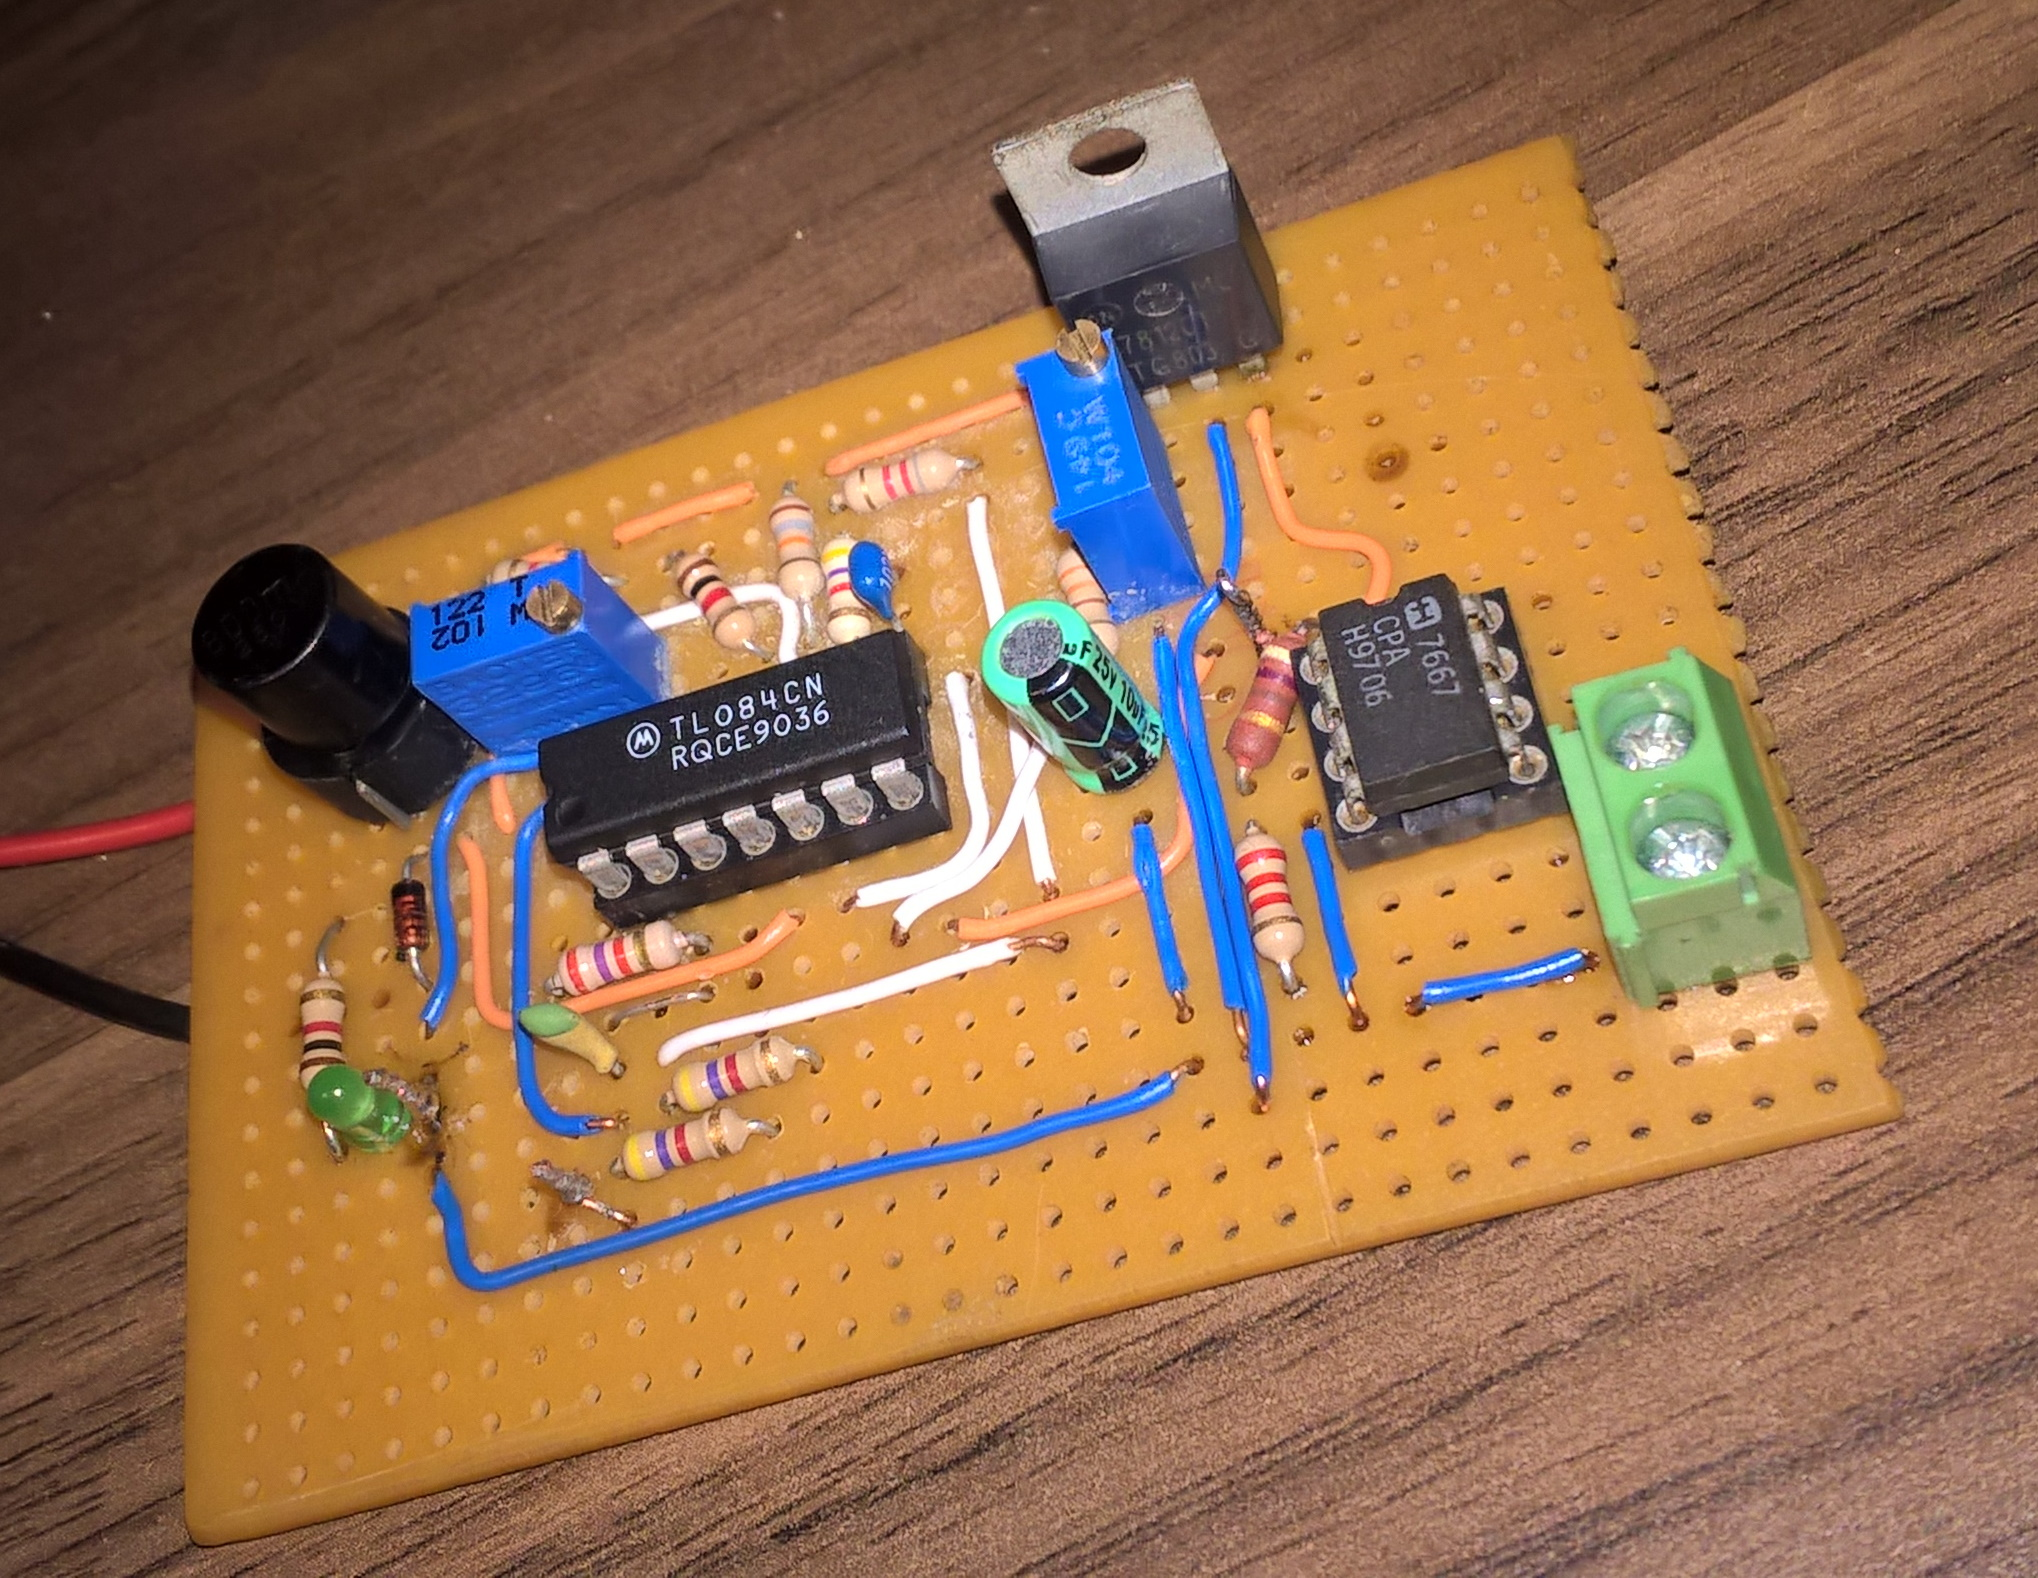
\includegraphics[scale=0.1]{./image/DevBoardPWM.jpg} \hspace{0.2cm}
	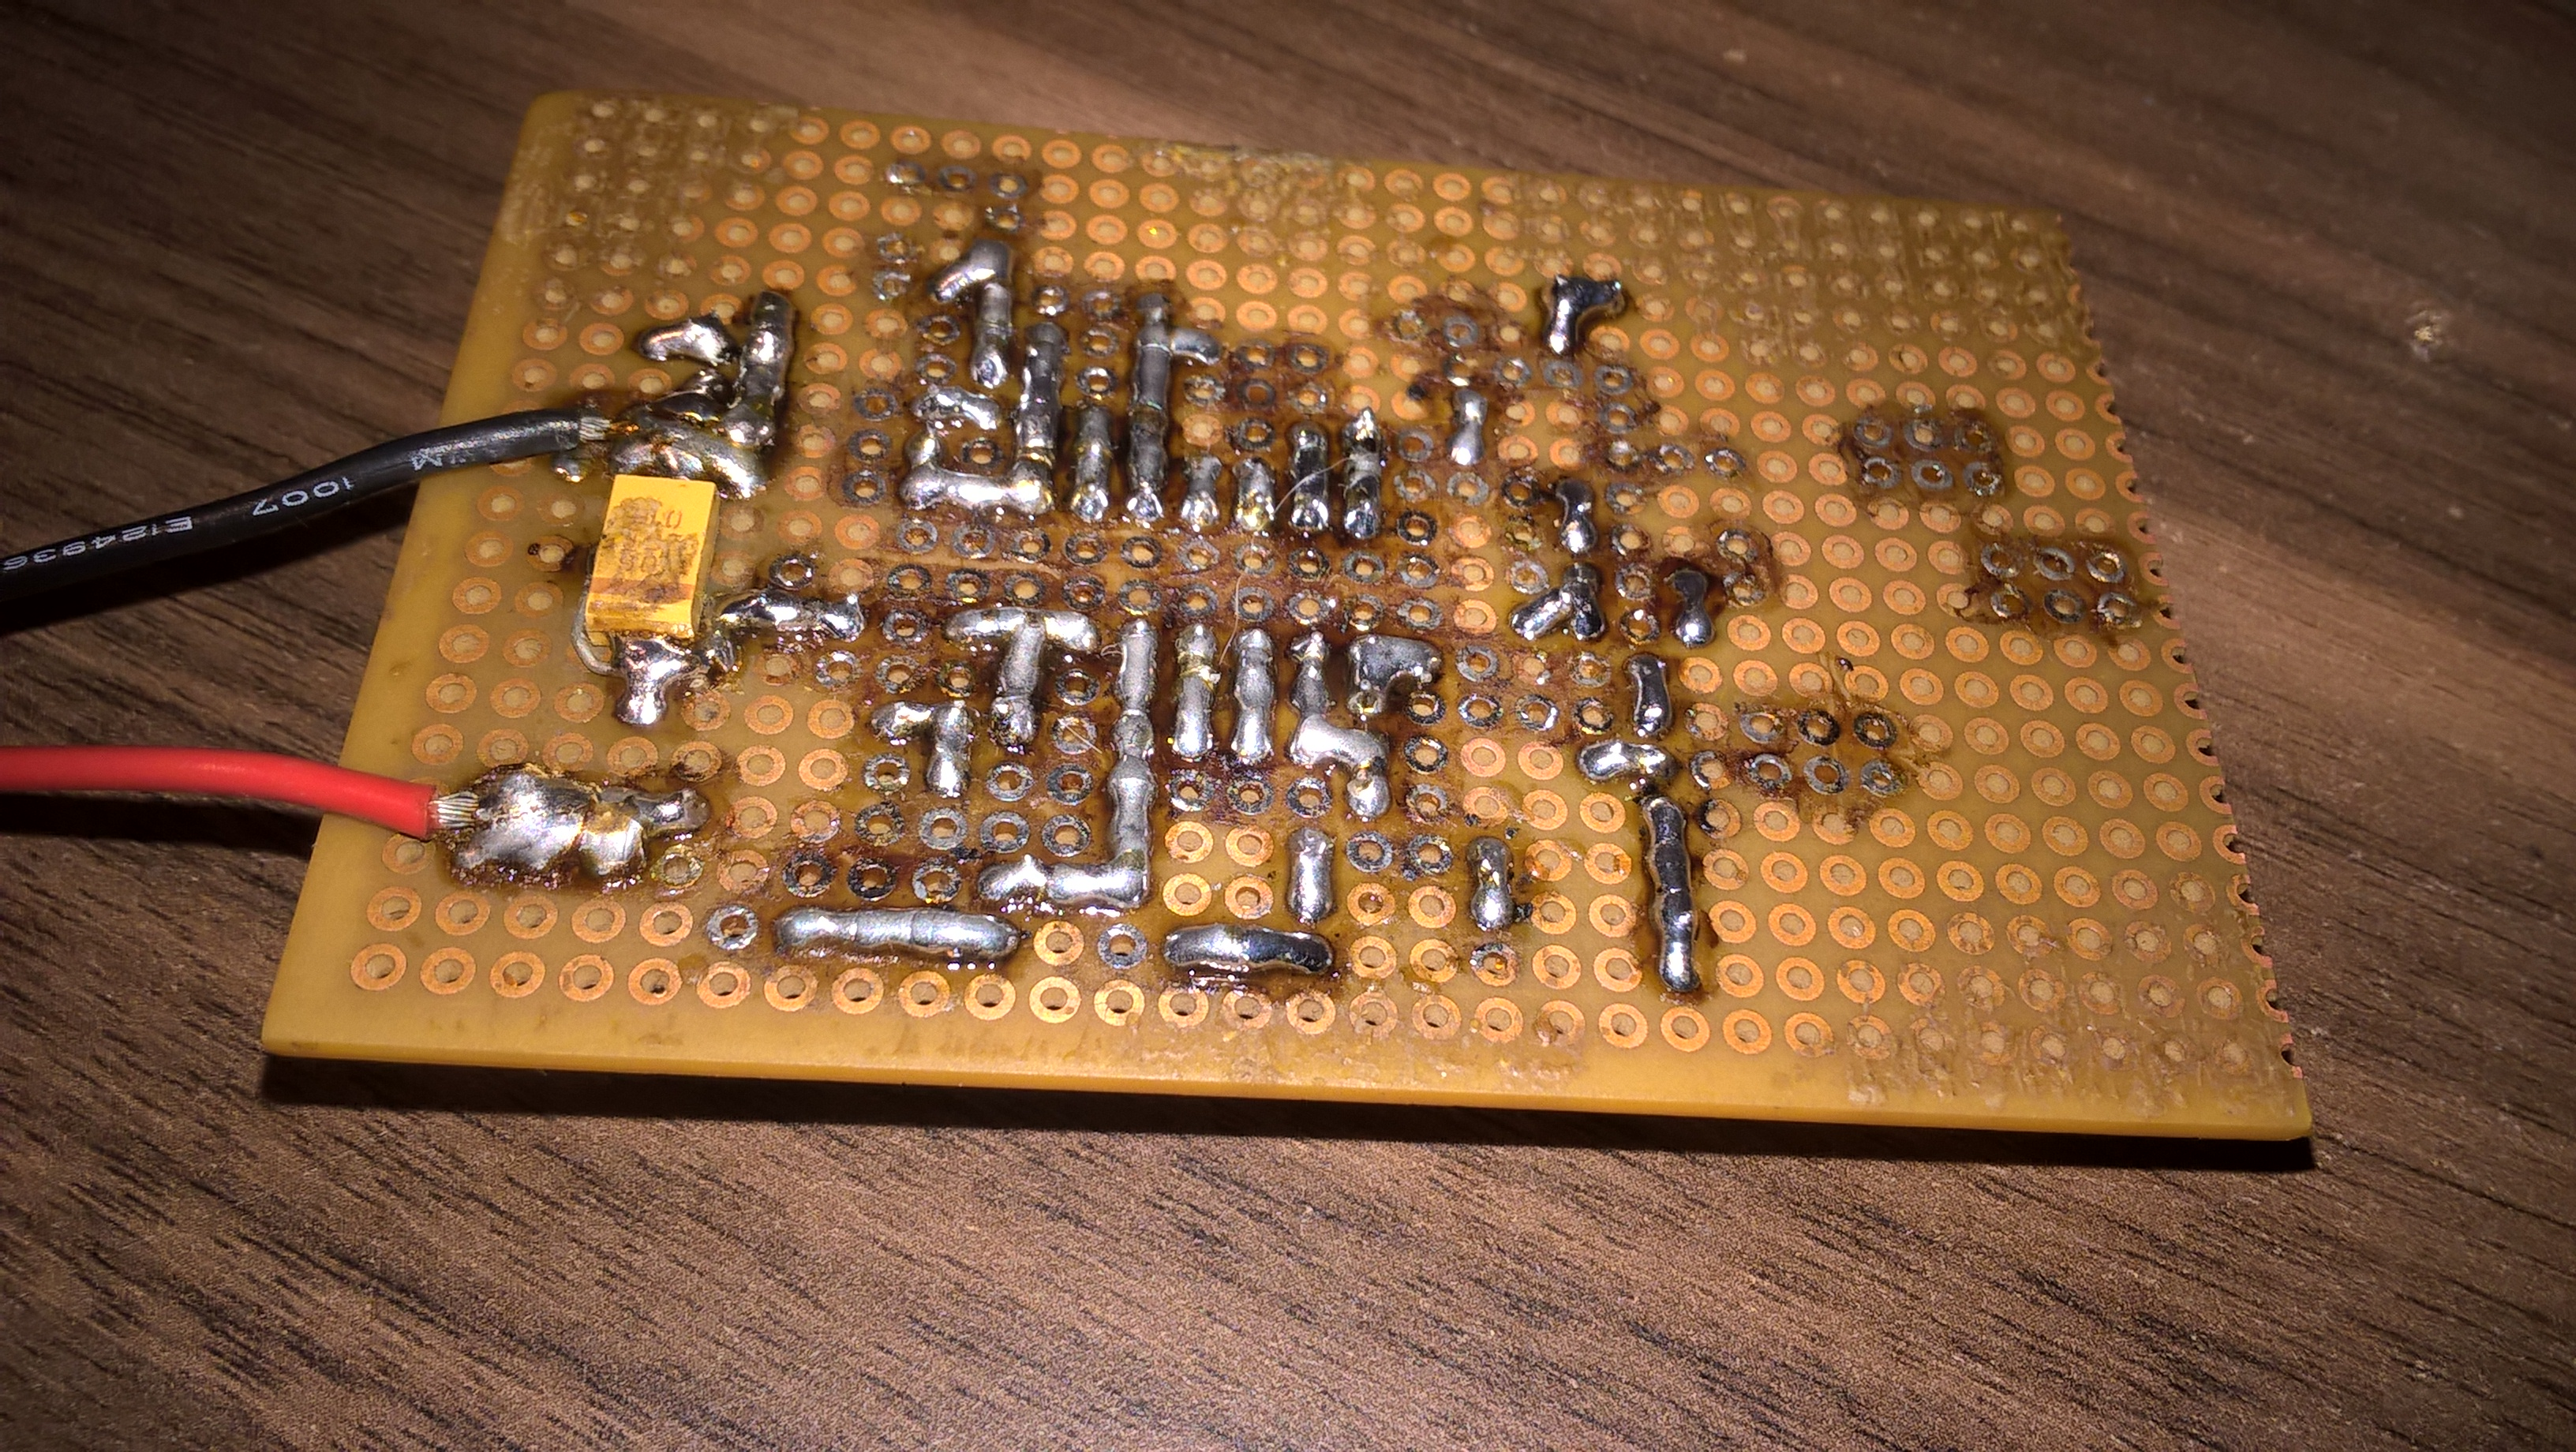
\includegraphics[scale=0.07]{./image/placa_2.jpg}
\end{center}
\caption{PCB}
\end{figure}\par
Este circuito tem um comportamento muito estável e flexibilidade, temos de ter em conta as características dos componentes, que não interfere na sua funcionalidade mas na tolerância que é dependente da temperatura, alimentação e dos componentes, se se quer grande precisão só através de medição e ajustes.
%%%%%%%%%%%%%%%%%%%%%%%%%%%%%%%%%%%%%%%%%%%%%%%%%%%%%%%%%%%%%%%%%%%%%%%%%%%
\section{Simulação}
%\begin{comment}	
\begin{figure}[H]
	\centering
	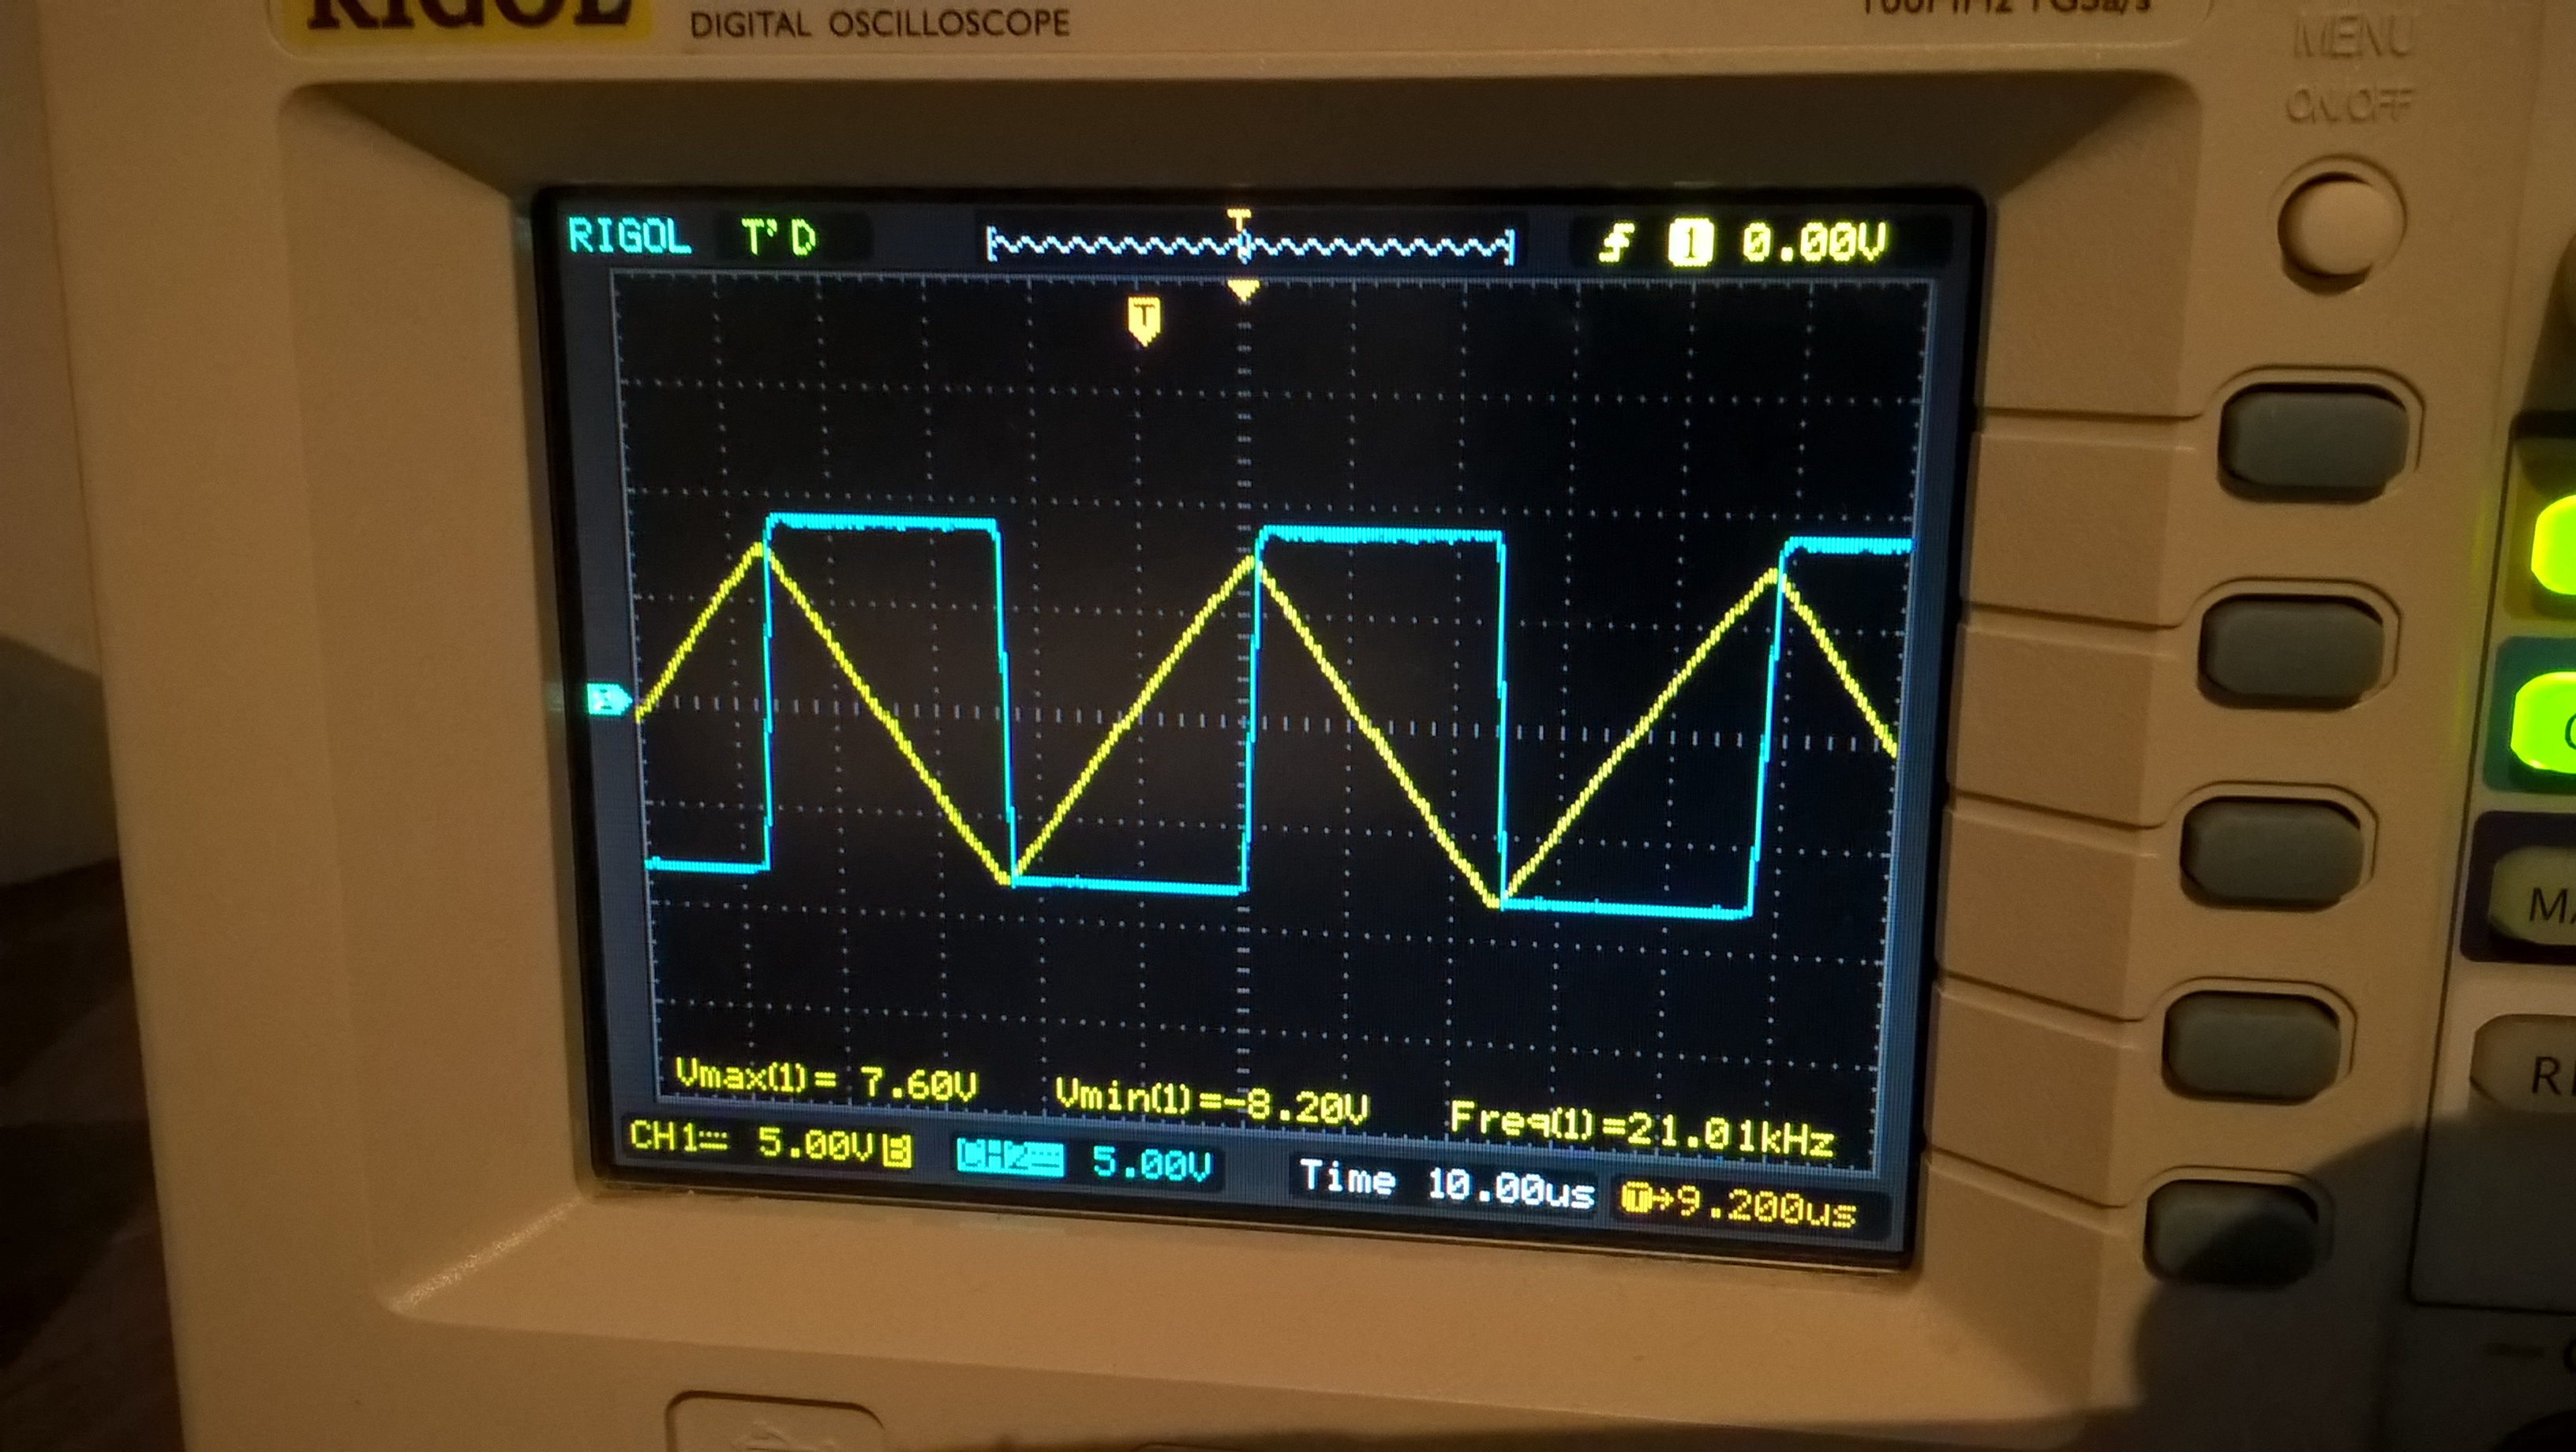
\includegraphics[scale=0.13]{./image/Ondas.jpg}\\
	\caption{Ondas}
\end{figure}
%\end{comment}
\newpage
%%%%%%%%%%%%%%%%%%%%%%%%%%%%%%%%%%%%%%%%%%%%%%%%%%%%%%%%%%%%%%%%%%%%%%%%%%%
\newpage
\footnote{Apontamentos}
%
	\end{document}
%%%%%%%%%%%%%%%%%%%%%%%%%%%%%%%%%EOF%%%%%%%%%%%%%%%%%%%%%%%%%%%%%%%%%%%%%%%
\begin{comment}
\begin{figure}[H]
\centering
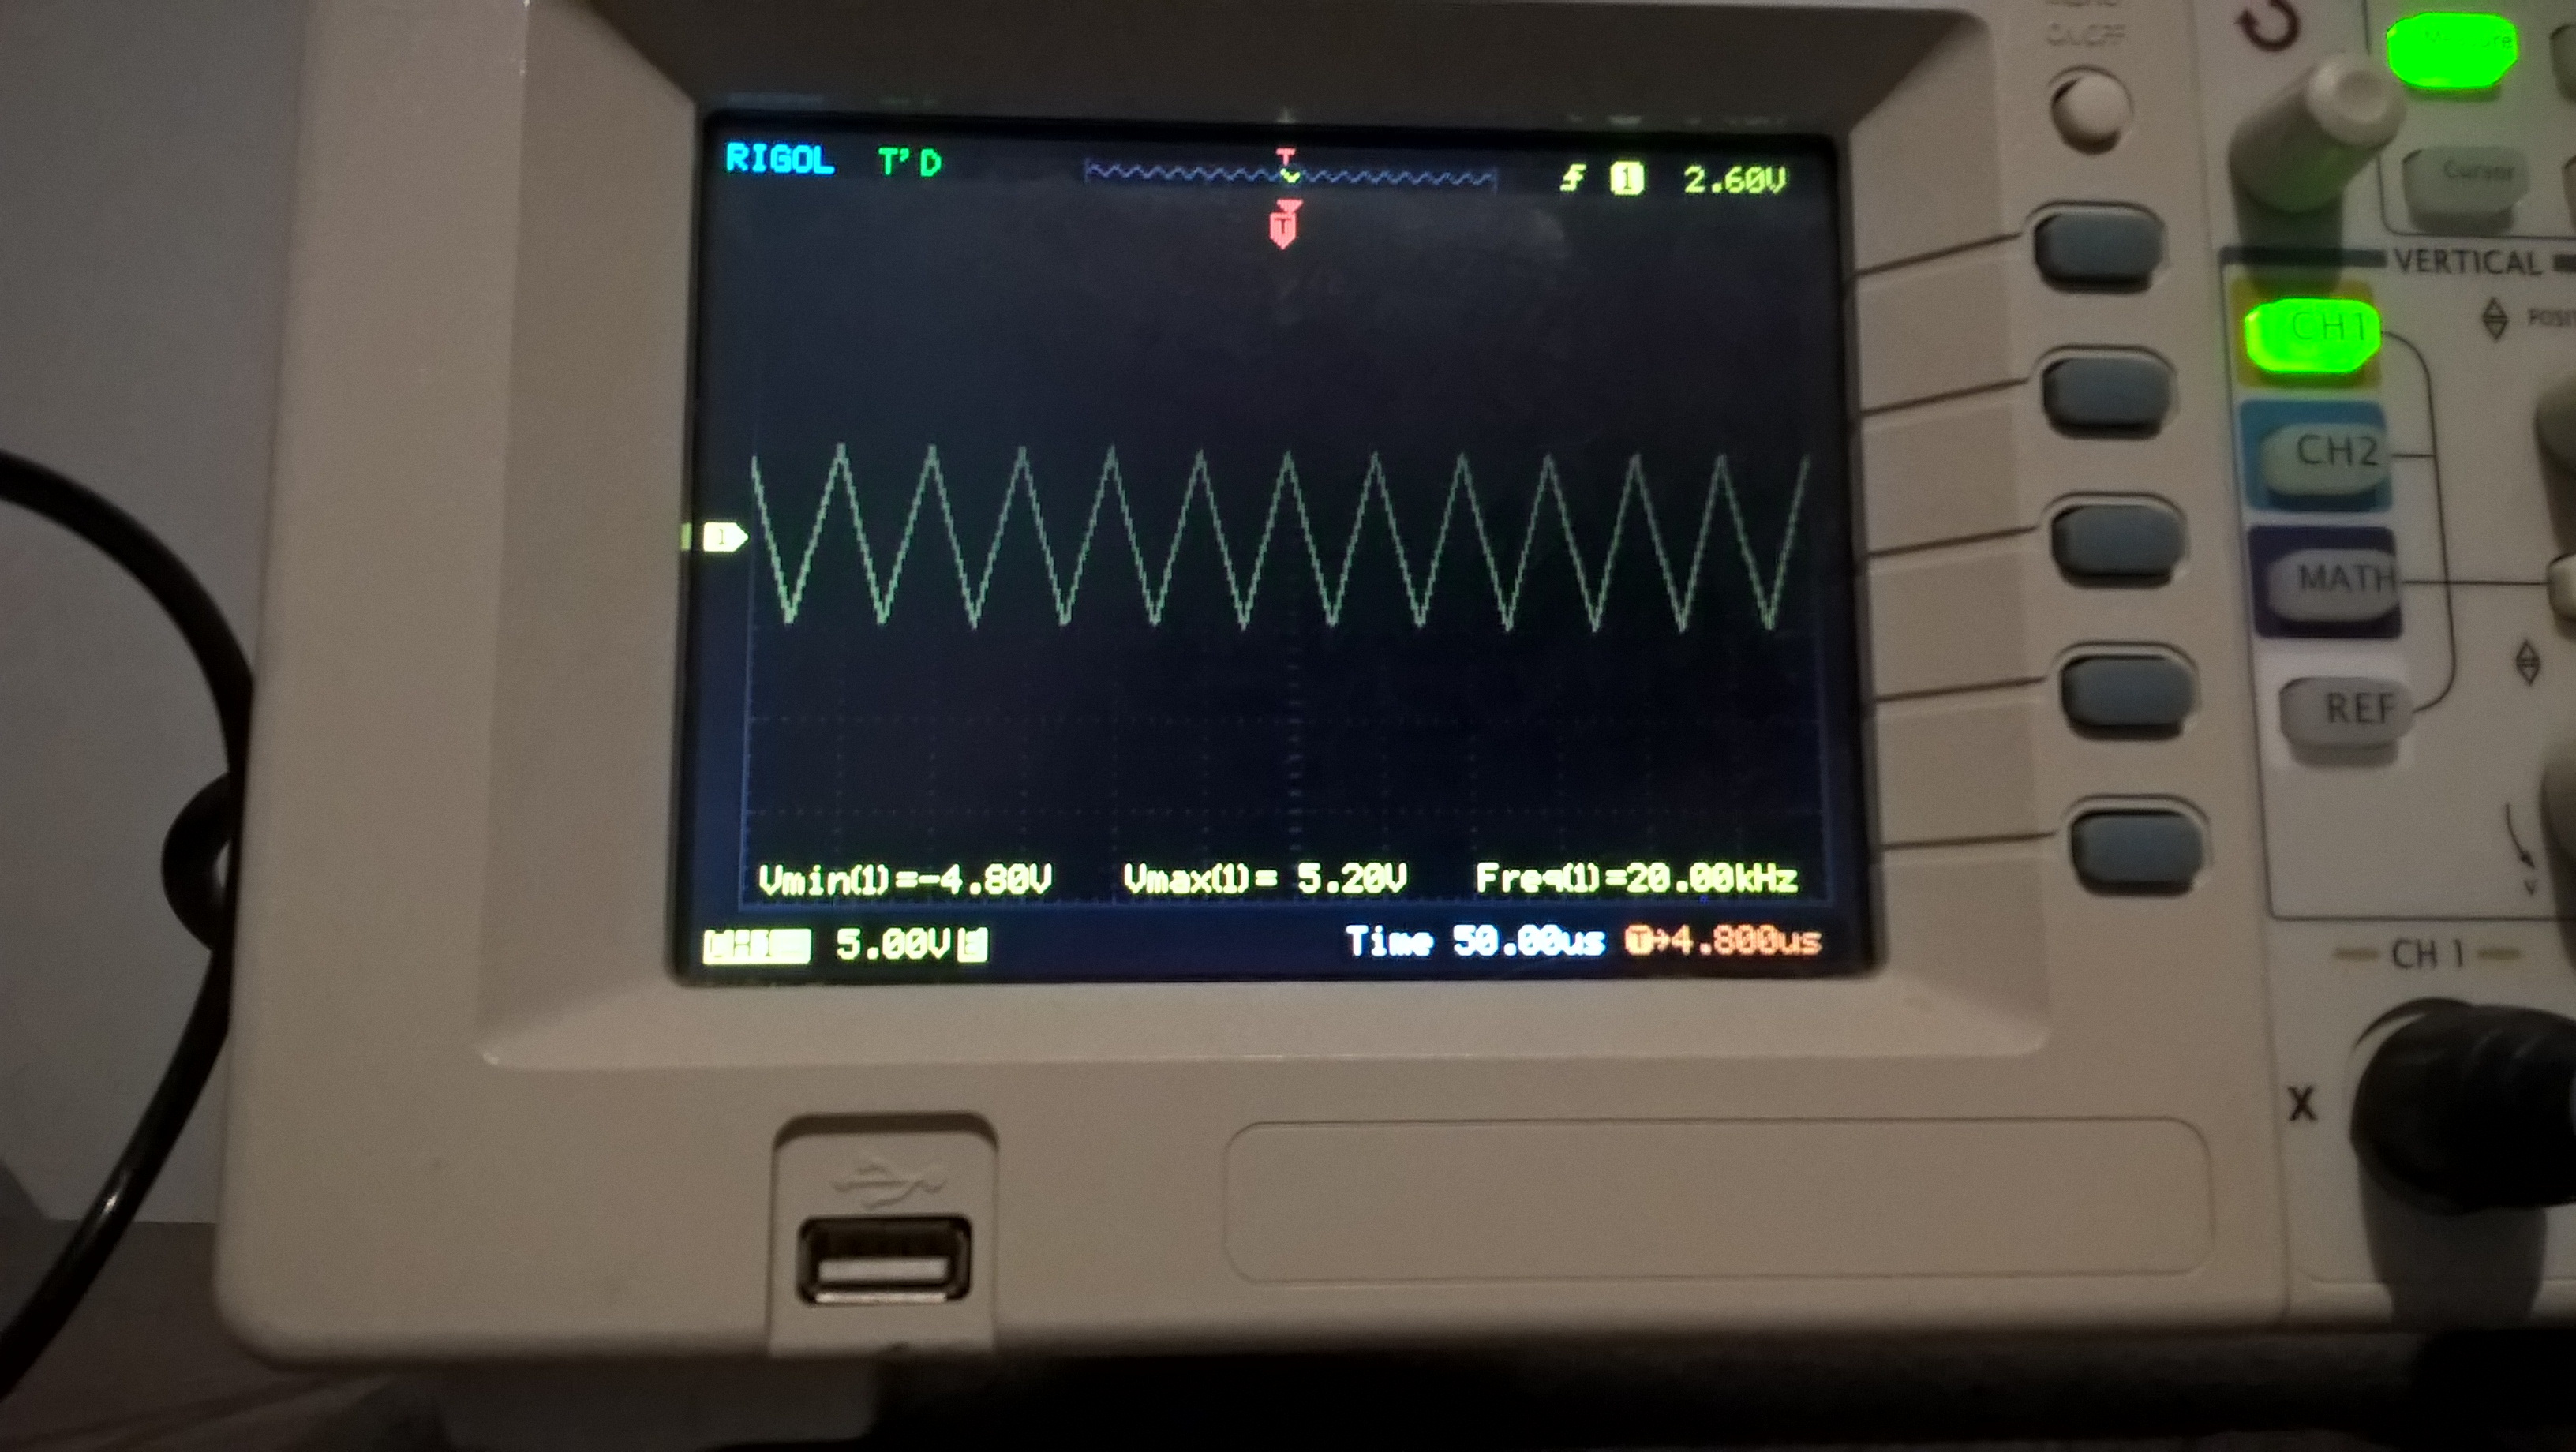
\includegraphics[scale=0.15]{./image/triangulo.jpg}\\
\caption{Onda Triangular}
\end{figure}\par
\end{comment}
%%%%%%%%%%%%%%%%%%%%%%%%%%%%%%%%%%%%%%%%%%%%%%%%%%%%%%%%%%%%%%%%%%%%%%%%%%%%